\documentclass[12pt, a4paper]{article} % Kelas standar artikel
\usepackage{../_internals/preamble_ui_ana} % Preamble baru kita

% --- Document Specific Information (from settings.tex or defined here) ---
% %-----------------------------------------------------------------------------%
% Informasi Mengenai Dokumen
%-----------------------------------------------------------------------------%
%
% Judul laporan.
\var{\judul}{Implementasi dan Analisis Efektivitas Vxlang \f{Code Virtualization} dalam mempersulit \f{Reverse Engineering}}
%
% Tulis kembali judul laporan, kali ini akan diubah menjadi huruf kapital
\Var{\Judul}{Implementasi dan Analisis Efektivitas Vxlang \f{Code Virtualization} dalam mempersulit \f{Reverse Engineering}}
%
% Tulis kembali judul laporan namun dengan bahasa Ingris
\var{\judulInggris}{Implementation and Analysis of the Effectiveness of Vxlang Code Virtualization in complicating Reverse Engineering}
%
% Tipe laporan, dapat berisi Skripsi, Tugas Akhir, Thesis, atau Disertasi
\var{\type}{Skripsi}
%
% Tulis kembali tipe laporan, kali ini akan diubah menjadi huruf kapital
\Var{\Type}{Skripsi}
%
% Tulis nama penulis
\var{\penulis}{Seno Pamungkas Rahman}
%
% Tulis kembali nama penulis, kali ini akan diubah menjadi huruf kapital
\Var{\Penulis}{Seno Pamungkas Rahman}
%
% Tulis NPM penulis
\var{\npm}{2106731586}
%
% Tuliskan Fakultas dimana penulis berada
\Var{\Fakultas}{Teknik}
\var{\fakultas}{Teknik}
%
% Tuliskan Program Studi yang diambil penulis
\Var{\Program}{Teknik Komputer}
\var{\program}{Teknik Komputer}
%
% Tuliskan tahun publikasi laporan
\Var{\bulan}{Mei}
\Var{\tahun}{2025}
%
% Tuliskan gelar yang akan diperoleh dengan menyerahkan laporan ini
\var{\gelar}{Sarjana Teknik}
%
% Tuliskan tanggal pengesahan laporan, waktu dimana laporan diserahkan ke
% penguji/sekretariat
\var{\tanggalPengesahan}{24 Mei 2025}
%
% Tuliskan tanggal keputusan sidang dikeluarkan dan penulis dinyatakan
% lulus/tidak lulus
\var{\tanggalLulus}{24 Mei 2025}
%
% Tuliskan pembimbing
\var{\pembimbing}{Dr. Ruki Harwahyu, S.T. M.T. MSc.}
%
% Tuliskan penguji
\var{\pengujisatu}{Yan Maraden, S.T., M.T., M.Sc.}
\var{\pengujidua}{Muhammad Firdaus Syawaludin Lubis, S.T., MT., Ph.D.}
%
% Alias untuk memudahkan alur penulisan paa saat menulis laporan
\var{\saya}{Penulis}

%-----------------------------------------------------------------------------%
% Judul Setiap Bab
%-----------------------------------------------------------------------------%
%
% Berikut ada judul-judul setiap bab.
% Silahkan diubah sesuai dengan kebutuhan.
%
\Var{\kataPengantar}{Kata Pengantar}
\Var{\babSatu}{Pendahuluan}
\Var{\babDua}{Tinjauan Pustaka}
\Var{\babTiga}{Metode Penelitian}
\Var{\babEmpat}{Implementasi}
\Var{\babLima}{Hasil Penelitian}
\Var{\babEnam}{Kesimpulan dan Saran}
 % Keep if settings.tex contains commands needed ONLY here (like \judul)
                      % If commands like \Penulis are only for skripsi, remove this input.

% Define commands specifically for THIS journal paper:
\newcommand{\journalTitle}{Implementation and Analysis of Code Virtualization Effectiveness using VxLang for Mitigating Reverse Engineering}
\newcommand{\authorOne}{Seno Pamungkas Rahman}
\newcommand{\authorOneAffiliation}{Department of Electrical Engineering, Faculty of Engineering, Universitas Indonesia, Depok, 16424, Indonesia} % Added postal code
\newcommand{\authorOneEmail}{seno.pamungkas@ui.ac.id}
% \newcommand{\authorTwo}{Dr. Ruki Harwahyu, S.T., M.T., M.Sc.} % Example for Advisor
% \newcommand{\authorTwoAffiliation}{Dept. of Electrical Engineering, Fac. of Engineering, Universitas Indonesia} % Keep affiliations consistent
% \newcommand{\authorTwoEmail}{ruki.harwahyu@ui.ac.id} % Example email
\newcommand{\correspondingAuthor}{Seno Pamungkas Rahman}


 % Variabel khusus dokumen ini

\addbibresource{../../pustaka.bib} % Path ke file .bib utama Anda

\begin{document}

% --- Blok Judul dan Penulis ---
% journal_ui_ana/indonesia/src/00_judul_penulis_blok.tex
\begin{center}
    \fontsize{14}{17}\selectfont\textbf{\myJudulIndonesia} % Times New Roman 14, centered, Bold
    \vspace{0.8cm}

    \fontsize{12}{14.4}\selectfont % Times New Roman 12
    \myPenulis, \myPembimbing \\
    \vspace{0.3cm}
    \myDepartment \\
    \myFaculty, \myUniversity, \myAddress \\
    \vspace{0.3cm}
    E-mail: \myEmail
\end{center}


% --- Abstrak Indonesia ---
\begin{singlespace} % Spasi 1 untuk blok abstrak
    % journal_ui_ana/indonesia/src/01_abstrak_indonesia.tex
\begin{center}
    \fontsize{12}{14.4}\selectfont\textbf{Abstrak} % Times New Roman 12, Bold
\end{center}
\fontsize{10}{12}\selectfont % Times New Roman 10, Spasi 1
Rekayasa balik merupakan ancaman serius terhadap keamanan perangkat lunak, memungkinkan penyerang untuk menganalisis, memahami, dan memodifikasi kode program tanpa izin. Teknik \f{obfuscation}, terutama virtualisasi kode, menjadi solusi yang menjanjikan untuk melindungi perangkat lunak dari ancaman ini. Penelitian ini bertujuan untuk mengimplementasikan dan menganalisis efektivitas virtualisasi kode dalam meningkatkan keamanan perangkat lunak dengan mempersulit rekayasa balik. Penelitian ini menggunakan VxLang sebagai platform virtualisasi kode. Metode penelitian yang digunakan meliputi implementasi virtualisasi kode pada sebuah aplikasi studi kasus, kemudian dilakukan analisis statis dan dinamis terhadap aplikasi sebelum dan sesudah di-\f{obfuscate}. Analisis statis dilakukan dengan membandingkan tingkat kesulitan dalam memahami kode \f{assembly} yang dihasilkan. Analisis dinamis dilakukan dengan mengukur waktu eksekusi dan sumber daya yang digunakan oleh aplikasi. Hasil penelitian menunjukkan bahwa virtualisasi kode dengan VxLang efektif dalam meningkatkan keamanan perangkat lunak. Kode yang telah di-\f{obfuscate} menjadi lebih sulit dipahami dan dianalisis, terlihat dari meningkatnya kompleksitas kode \f{assembly}. Penelitian ini diharapkan dapat membuktikan bahwa virtualisasi kode dengan VxLang merupakan teknik yang efektif untuk melindungi perangkat lunak dari rekayasa balik dan dapat dipertimbangkan sebagai solusi untuk meningkatkan keamanan aplikasi.
\vspace{0.5cm}

\end{singlespace}

% --- Judul Inggris ---
% journal_ui_ana/indonesia/src/02_title_english.tex
\begin{center}
    \fontsize{12}{14.4}\selectfont\textbf{\myTitleEnglish} % Times New Roman 12, Bold
\end{center}

% --- Abstrak Inggris ---
\begin{singlespace} % Spasi 1 untuk blok abstrak
    \begin{center}
    \fontsize{12}{14.4}\selectfont\textbf{Abstract} % Times New Roman 12, Bold
\end{center}
\fontsize{10}{12}\selectfont % Times New Roman 10, Spasi 1
Reverse engineering is a serious threat to software security, allowing attackers to analyze, understand, and modify program code without permission. Obfuscation techniques, especially code virtualization, are promising solutions to protect software from this threat. This study aims to implement and analyze the effectiveness of code virtualization in improving software security by complicating reverse engineering. This study uses VxLang as a code virtualization platform. The research methods used include implementing code virtualization on a case study application, then conducting static and dynamic analysis of the application before and after obfuscation. Static analysis is done by comparing the level of difficulty in understanding the resulting assembly code. Dynamic analysis is done by measuring the execution time and resources used by the application. The results of the study show that code virtualization with VxLang is effective in improving software security. Obfuscated code becomes more difficult to understand and analyze, as seen from the increasing complexity of the assembly code. This study is expected to prove that code virtualization with VxLang is an effective technique to protect software from reverse engineering and can be considered as a solution to improve application security.
\vspace{0.5cm}

\end{singlespace}

% --- Keywords ---
% journal_ui_ana/indonesia/src/04_keywords_english.tex
\noindent % Agar tidak indentasi
\fontsize{10}{12}\selectfont\textit{Keywords: Code Obfuscation, Code Virtualization, Software Protection, Reverse Engineering, Security Analysis, Performance Overhead} % Menambahkan dari keywords IEEE journal untuk kelengkapan


\vspace{1cm} % Spasi sebelum konten utama

% --- Konten Utama ---
\onehalfspacing % Spasi 1.5 untuk konten utama (TNR 12 dari class)

% journal_ui_ana/indonesia/src/10_pendahuluan.tex
\section{Pendahuluan}
Perkembangan pesat teknologi perangkat lunak telah mendorong terciptanya aplikasi yang semakin kompleks, namun diiringi oleh peningkatan ancaman keamanan. Rekayasa balik (\f{reverse engineering}), proses menganalisis perangkat lunak untuk memahami cara kerjanya tanpa akses ke kode sumber \cite{Has18}, merupakan kerentanan kritis. Penyerang memanfaatkan rekayasa balik untuk mengungkap algoritma, menemukan celah keamanan, membajak perangkat lunak, dan menyisipkan kode berbahaya \cite{Wak24}. Ukuran keamanan tradisional seringkali tidak memadai terhadap analisis logika program saat berjalan \cite{Sec19}.

Untuk mengatasi ancaman ini, teknik pengaburan kode (\f{code obfuscation}) bertujuan mengubah kode program menjadi bentuk yang lebih sulit dipahami tanpa mengubah fungsionalitasnya \cite{Jin24}. Di antara berbagai strategi pengaburan, virtualisasi kode (\f{code virtualization}) menonjol sebagai pendekatan yang sangat kuat \cite{Ore06, Zho24}. Teknik ini menerjemahkan kode mesin asli menjadi instruksi \f{bytecode} khusus yang dieksekusi oleh mesin virtual (VM) yang tertanam dalam aplikasi \cite{Don20}. Arsitektur Set Instruksi (ISA) unik dari VM ini membuat alat rekayasa balik konvensional seperti \f{disassembler} dan \f{debugger} menjadi tidak efektif karena tidak dapat langsung menginterpretasikan kode yang divirtualisasi \cite{Salwan2018SymbolicDeobfuscation}. Penyerang harus terlebih dahulu menguraikan arsitektur VM dan \f{bytecode}-nya, yang secara substansial meningkatkan upaya dan kompleksitas analisis \cite{Hac24}.

VxLang adalah sebuah kerangka kerja proteksi kode yang menggabungkan kapabilitas virtualisasi kode, menargetkan \f{executable} Windows PE \cite{VxLang}. Kerangka kerja ini menyediakan mekanisme untuk mentransformasi kode asli menjadi format \f{bytecode} internalnya, yang dieksekusi oleh VM yang tersemat. Memahami efektivitas praktis dan biaya terkait dari alat semacam itu sangat penting bagi pengembang yang mencari solusi proteksi perangkat lunak yang tangguh.

Makalah ini menyelidiki efektivitas virtualisasi kode menggunakan VxLang dalam mengurangi upaya rekayasa balik. Kami bertujuan untuk menjawab pertanyaan kunci berikut:
\begin{enumerate}
    \item Seberapa efektif virtualisasi kode VxLang mengaburkan logika program terhadap teknik rekayasa balik statis dan dinamis?
    \item Apa dampak kuantitatif dari virtualisasi VxLang terhadap performa aplikasi (waktu eksekusi) dan ukuran berkas?
\end{enumerate}

Untuk menjawab pertanyaan-pertanyaan ini, kami mengimplementasikan virtualisasi VxLang pada fungsi-fungsi terpilih dalam aplikasi studi kasus (mensimulasikan autentikasi) dan \f{benchmark} performa (QuickSort, enkripsi AES). Kami kemudian melakukan analisis statis komparatif (menggunakan Ghidra \cite{Nat19}) dan analisis dinamis (menggunakan x64dbg \cite{Dun14}) pada biner asli dan yang telah divirtualisasi. \f{Overhead} performa diukur dengan membandingkan waktu eksekusi dan ukuran \f{executable}, dan dampak pada alat deteksi \f{malware} otomatis dinilai menggunakan analisis VirusTotal pada studi kasus yang relevan.

Kontribusi utama dari penelitian ini adalah:
\begin{itemize}
    \item Implementasi dan evaluasi praktis virtualisasi kode VxLang pada segmen kode representatif.
    \item Analisis kualitatif dan kuantitatif terhadap peningkatan kesulitan yang ditimbulkan pada rekayasa balik statis dan dinamis oleh VxLang.
    \item Pengukuran dan analisis terhadap \f{overhead} performa dan ukuran berkas yang terkait dengan virtualisasi VxLang.
    \item Penilaian empiris terhadap \textit{trade-off} keamanan-performa yang ditawarkan oleh kerangka kerja VxLang.
\end{itemize}

Sisa dari makalah ini diorganisasikan sebagai berikut: Bagian selanjutnya membahas penelitian terkait dalam pengaburan dan virtualisasi kode. Kemudian, metodologi yang digunakan dalam eksperimen kami dirinci. Setelah itu, detail implementasi diuraikan secara singkat. Selanjutnya, hasil eksperimental untuk analisis keamanan dan performa disajikan dan dibahas. Akhirnya, makalah ini ditutup dengan kesimpulan dan saran untuk penelitian di masa mendatang.

% Ganti nama file berikut sesuai dengan struktur yang Anda inginkan,
% ini hanya contoh berdasarkan PDF dan file Anda yang ada
% journal_ui_ana/english/src/20_pengembangan_hipotesis.tex
% This can be named 20_literature_review.tex or 20_related_work.tex if more appropriate
\section{Literature Review and Theoretical Background} % Title adjusted to be more general for a journal

Reverse engineering is a fundamental process in software analysis aimed at understanding the internal mechanisms of a system without access to its original source code \cite{Has18, gee24}. This process poses a significant threat to software security as it can be exploited to uncover proprietary algorithms, identify security vulnerabilities, pirate licenses, and even inject malicious code \cite{Wak24}. This vulnerability has driven the development of various protection techniques, including code obfuscation.

\subsection{Code Obfuscation Techniques}
Code obfuscation aims to transform program code into a functionally equivalent form that is significantly more difficult for humans to understand and analyze \cite{Jin24}. The goal is not to make reverse engineering impossible, but to increase the complexity and cost required, making it impractical for attackers. Obfuscation techniques can be classified based on the level of abstraction at which they are applied:

\subsubsection{Source Code Obfuscation}
Modifications are made to human-readable source code.
\begin{itemize}
    \item \bo{Layout Obfuscation:} Alters code appearance, such as scrambling variable and function names \cite{Cha04}, and removing whitespace and comments \cite{Bal11}. Provides minimal security against automated analysis.
    \item \bo{Data Obfuscation:} Hides data representation, for example, through string encoding \cite{Ert05, Fuk08, Kov13}, instruction substitution \cite{LeD12, Dar10}, or using mixed boolean-arithmetic expressions \cite{Liu21, Sch22, Zho07} to disguise data manipulation logic.
    \item \bo{Control Flow Obfuscation:} Modifies the program's execution path logic. Examples include inserting bogus control flow \cite{LiY211}, using opaque predicates \cite{XuD16}, and control flow flattening, which transforms structured code into a large and complex \code{switch} statement \cite{Lás09}.
\end{itemize}

\subsubsection{Bytecode Obfuscation}
This technique targets intermediate code such as Java bytecode, .NET CIL, or LLVM IR. Methods include identifier renaming, control flow obfuscation, string encryption, and inserting dummy code \cite{Pie18, Yak20}. Effective in complicating decompilation back to high-level source code.

\subsubsection{Binary Code Obfuscation}
Operates directly on machine-executable code.
\begin{itemize}
    \item \bo{Code Packing/Encryption:} Compresses or encrypts the original code, requiring a runtime stub to unpack/decrypt the code before execution \cite{Rou13}. Primarily hinders static analysis, but the original code is revealed in memory during execution.
    \item \bo{Control Flow Manipulation:} Uses indirect jumps/calls, modifies \code{call}/\code{ret} instructions, or breaks code into small blocks with jumps to disrupt linear disassembly and analysis \cite{Rou13}.
    \item \bo{Constant Obfuscation:} Hides constant values through arithmetic or logical operations \cite{Rou13}.
    \item \bo{Code Virtualization:} Considered one of the strongest binary obfuscation techniques, discussed further below.
\end{itemize}

\subsection{Code Virtualization (VM-Based Obfuscation)}
Code virtualization, or Virtual Machine (VM)-based obfuscation, is an advanced technique where segments of native machine code are translated into a custom bytecode format. This bytecode is then executed by a specially designed VM embedded directly into the application \cite{Ore06, Zho24}. As illustrated in Figure \ref{fig:jurnal_ui_ana_virtualization_process} from Oreans' research \cite{Ore06}, this process transforms the original code into a series of virtual instructions.

\begin{figure}[H]
	\centering
	\includegraphics[width=0.7\textwidth]{\Assets/code_virtualization_process.png} % Assuming Assets is defined or path adjusted
	\caption{Code Virtualization Process \cite{Ore06}}
	\label{fig:jurnal_ui_ana_virtualization_process_en} % Unique label for the English journal
\end{figure}

The abstraction layer introduced by this VM creates a significant barrier for reverse engineers. Standard analysis tools cannot directly interpret the unique bytecode ISA \cite{Salwan2018SymbolicDeobfuscation}. Reverse engineers must first understand the VM's architecture, virtual instruction handler implementations, and bytecode mapping, a complex and time-consuming task \cite{Don20, Hac24}.

Key aspects of VM-based obfuscation include:
\begin{itemize}
    \item \bo{Custom ISA:} Each protected application can potentially have a unique or mutated set of virtual instructions, hindering signature-based detection or reuse of analysis results. Oreans \cite{Ore06} highlights the possibility of generating diverse VMs for different protected copies of an application.
    \item \bo{VM Architecture:} Typical VM components include fetch, decode, dispatch, and handler units, mimicking CPU operations but implemented in software \cite{Salwan2018SymbolicDeobfuscation, Hac24}. The complexity and implementation details of these handlers directly impact both security and performance. The execution flow of code virtualization can be seen in Figure \ref{fig:jurnal_ui_ana_execution_virtualization_en} (adapted from \cite{Don20}).

    \begin{figure}[H]
        \centering
        \includegraphics[width=0.6\textwidth]{\Assets/virtualization_execution.png}
        \caption{Code Virtualization Execution Flow (adapted from \cite{Don20})}
        \label{fig:jurnal_ui_ana_execution_virtualization_en}
    \end{figure}

    \item \bo{Security vs. Performance Trade-off:} The interpretation layer introduced by the VM inherently adds performance overhead compared to native execution. The level of obfuscation within the VM handlers and the complexity of the virtual instructions influence this trade-off.
\end{itemize}

Several commercial tools like VMProtect \cite{VMP24} and Themida \cite{Ore24} (which also includes virtualization features beyond basic packing) employ code virtualization. Academic research has also explored techniques such as symbolic deobfuscation to analyze virtualized code \cite{Salwan2018SymbolicDeobfuscation} and methods to enhance virtualization robustness, such as virtual code folding \cite{Don20}.

\subsection{Disassembly Techniques and Challenges}
Understanding the efficacy of binary obfuscation, particularly code virtualization, necessitates a brief overview of disassembly techniques. Disassemblers translate machine code into human-readable assembly language, forming a cornerstone of reverse engineering \cite{Sikorski2012}.

\subsubsection{Static Disassemblers}
Static disassemblers, such as Ghidra \cite{Nat19} and IDA Pro \cite{Hex91}, analyze executable files without running them. They employ techniques like linear sweep or recursive traversal to identify instruction sequences \cite{Eilam2011, Ko2007}. While comprehensive, static analysis struggles with code that is encrypted, packed, self-modifying, or significantly transformed, as the disassembler may misinterpret data as code or fail to follow the true control flow \cite{Sikorski2012, Blazytko2017}. Crucially, when faced with custom bytecode from a VM, static disassemblers designed for standard ISAs (e.g., x86-64) cannot correctly interpret these non-native instructions, leading to analysis failure.

\subsubsection{Dynamic Disassemblers}
Dynamic disassembly, typically a feature of debuggers like x64dbg \cite{Dun14}, occurs during program execution. The debugger disassembles instructions on-the-fly as they are about to be executed by the CPU. This approach can overcome some static analysis limitations, such as revealing unpacked or decrypted code in memory \cite{Sikorski2012}. Debuggers can also access runtime symbol information loaded by the operating system for system libraries, providing context for API calls. However, while a debugger can step through the native instructions of an embedded VM's interpreter, it will not directly reveal the original, pre-virtualized logic of the application. Instead, it shows the VM's internal operations executing the custom bytecode, which still obscures the application's core semantics from the analyst. These inherent limitations of standard disassembly tools underscore the challenge posed by advanced obfuscation techniques like code virtualization.

\subsection{VxLang in Context}
VxLang positions itself as a comprehensive framework offering binary protection, code obfuscation (including flattening), and code virtualization \cite{VxLang}. Its approach involves transforming native x86-64 code into an internal bytecode executed by its VM. This study aims to provide an empirical evaluation of the effectiveness of VxLang's virtualization component against standard reverse engineering practices and quantify its associated performance costs, thereby contributing practical insights into its utility as a software protection mechanism. Unlike analyzing established commercial protectors, this research focuses on the specific implementation and impact of the VxLang framework.
 % atau tinjauan_pustaka.tex (related_work.tex)
% journal_ui_ana/indonesia/src/30_desain_penelitian.tex
\section{Desain Penelitian dan Metodologi} % Judul bisa disesuaikan, "Desain Penelitian" atau "Metodologi"

Penelitian ini menggunakan pendekatan eksperimental kuantitatif untuk mengevaluasi efektivitas virtualisasi kode menggunakan VxLang dalam mempersulit upaya rekayasa balik dan menganalisis \f{overhead} performa yang ditimbulkannya.

\subsection{Desain Eksperimen}
Desain eksperimen yang digunakan adalah perbandingan antara kelompok kontrol dan kelompok eksperimen.
\begin{itemize}
    \item \bo{Kelompok Kontrol:} Aplikasi studi kasus dan \f{benchmark} yang dikompilasi secara normal tanpa penerapan virtualisasi kode VxLang.
    \item \bo{Kelompok Eksperimen:} Aplikasi dan \f{benchmark} yang sama, namun bagian kode kritikalnya telah diproses menggunakan virtualisasi kode VxLang.
\end{itemize}
Variabel independen adalah penerapan virtualisasi kode VxLang, sedangkan variabel dependen meliputi tingkat kesulitan rekayasa balik (analisis statis dan dinamis) dan dampak performa (waktu eksekusi dan ukuran berkas).

\subsection{Objek Studi}
Objek studi dalam penelitian ini mencakup:
\begin{enumerate}
    \item \bo{Aplikasi Studi Kasus Autentikasi:} Aplikasi simulasi login pengguna dikembangkan dalam beberapa varian antarmuka (Konsol, Qt, Dear ImGui) dan dua mekanisme autentikasi (kredensial \f{hardcoded} dan validasi berbasis \f{cloud}). Aplikasi ini menjadi target utama analisis rekayasa balik.
    \item \bo{Aplikasi \f{Benchmark} Performa:} Aplikasi yang dirancang khusus untuk mengukur dampak performa pada tugas komputasi spesifik, yaitu algoritma QuickSort dan enkripsi AES-CBC-256. Sebuah aplikasi minimal dengan data tersemat juga digunakan untuk menilai peningkatan ukuran berkas dasar.
    \item \bo{Studi Kasus \f{Remote Administration Tool} (RAT):} Klien dari Lilith RAT \cite{LilithRAT}, sebuah RAT \f{open-source}, dianalisis untuk fungsionalitas pasca-virtualisasi dan perubahan profil deteksi pada VirusTotal. Sembilan sampel \f{malware}/PUA tambahan juga dianalisis dampaknya pada deteksi VirusTotal.
\end{enumerate}

\subsection{Instrumen dan Bahan Penelitian}
Penelitian ini menggunakan instrumen berikut:
\begin{itemize}
    \item \bo{Perangkat Keras:} PC berbasis Windows 11 (64-bit).
    \item \bo{Perangkat Lunak Pengembangan:} Clang/clang-cl (C++17), CMake, Ninja, VxLang SDK, Qt 6, Dear ImGui, OpenSSL 3.x, libcurl.
    \item \bo{Alat Analisis:} Ghidra (v11.x) untuk analisis statis, x64dbg (rilis terbaru) untuk analisis dinamis.
    \item \bo{Pengukuran Performa:} Pustaka C++ \code{std::chrono} untuk waktu, \code{std::filesystem::file\_size} untuk ukuran berkas.
\end{itemize}

\subsection{Prosedur Pengumpulan Data}
Pengumpulan data dilakukan melalui beberapa tahapan utama:

\subsubsection{Persiapan Artefak}
Aplikasi studi kasus dan \f{benchmark} dikompilasi dalam dua versi: asli (tanpa virtualisasi) dan \f{intermediate} (dengan makro VxLang dan tertaut pustaka VxLang). Versi \f{intermediate} kemudian diproses menggunakan \f{tool command-line} \code{vxlang.exe} untuk menghasilkan \f{executable} tervirtualisasi akhir (\code{*\_vxm.exe}).

\subsubsection{Analisis Keamanan}
Untuk setiap aplikasi autentikasi (asli dan tervirtualisasi):
\begin{enumerate}
    \item \bo{Analisis Statis (Ghidra):} Memuat \f{executable}, mencari \f{string} relevan (misalnya, "Gagal", "Sah", potensi kredensial), menganalisis \f{disassembly}/\f{decompilation} di sekitar referensi \f{string} atau titik masuk, mengidentifikasi lompatan kondisional yang mengontrol keberhasilan/kegagalan autentikasi, dan mencoba \f{patching} statis untuk mem-\textit{bypass} logika. Observasi sistematis dicatat.
    \item \bo{Analisis Dinamis (x64dbg):} Menjalankan \f{executable} di bawah \f{debugger}, mencari \f{string}/\f{pattern} saat \textit{runtime}, mengatur \f{breakpoint} pada lokasi logika yang dicurigai, melangkah melalui eksekusi, mengamati nilai register/memori, dan mencoba manipulasi \textit{runtime} (mem-\textit{patch} lompatan kondisional) untuk mem-\textit{bypass} autentikasi. Observasi sistematis dicatat.
\end{enumerate}
Diagram alir prosedur pengujian keamanan autentikasi dapat dilihat pada Gambar \ref{fig:flow_auth_test_proc_jurnal_ui_ana} (diadaptasi dari metodologi skripsi). % Menggunakan referensi ke gambar dari skripsi
% Anda dapat menyalin gambar relevan ke direktori assets jurnal dan merujuknya secara lokal jika perlu
% \begin{figure}[H]
% 	\centering
% 	\includegraphics[width=0.8\columnwidth]{\Assets/nama_diagram_alur_autentikasi.png}
% 	\caption{Diagram Alur Prosedur Pengujian Keamanan Autentikasi.}
% 	\label{fig:flow_auth_test_proc_jurnal_ui_ana}
% \end{figure}

\subsubsection{Analisis Performa}
Untuk setiap aplikasi \f{benchmark} (asli dan tervirtualisasi):
\begin{enumerate}
    \item \bo{Waktu Eksekusi:} Menjalankan \f{benchmark} QuickSort 100 kali per ukuran data, mencatat waktu individual. Menjalankan \f{benchmark} AES pada data 1GB, mencatat total waktu enkripsi/dekripsi. Menggunakan \code{std::chrono}. Menghitung rata-rata, standar deviasi (untuk QuickSort), dan \f{throughput} (untuk AES).
    \item \bo{Ukuran Berkas:} Mengukur ukuran \f{executable} akhir dalam \f{byte} menggunakan \code{std::filesystem::file\_size}.
\end{enumerate}

\subsubsection{Analisis Lilith RAT dan Sampel Malware Lainnya}
\begin{enumerate}
    \item \bo{Pengujian Integritas Fungsional (Lilith RAT):} Klien tervirtualisasi diuji untuk fungsionalitas inti RAT (koneksi ke server, eksekusi perintah jarak jauh, akses sistem berkas) terhadap server yang tidak dimodifikasi di jaringan lokal.
    \item \bo{Analisis VirusTotal:} Kedua versi (\f{executable} asli dan tervirtualisasi) dari klien Lilith RAT dan sembilan sampel \f{malware}/PUA lainnya diunggah ke VirusTotal untuk membandingkan tingkat deteksi dan karakterisasi ancaman.
\end{enumerate}

\subsection{Teknik Analisis Data}
\begin{itemize}
    \item \bo{Analisis Proteksi Keamanan:} Metrik kuantitatif (misalnya, tingkat keberhasilan \textit{bypass}, persentase \f{string} kritis yang berhasil diobfuskasi, pengurangan fungsi yang dapat diidentifikasi) dan analisis deskriptif dari observasi sistematis pada analisis statis dan dinamis.
    \item \bo{Data Performa:} Perhitungan statistik deskriptif, \f{overhead} persentase untuk waktu eksekusi, perhitungan \f{throughput} (MB/s), dan persentase peningkatan ukuran berkas. Tabel dan grafik komparatif akan digunakan.
    \item \bo{Analisis \textit{Trade-off}:} Sintesis temuan keamanan dan hasil performa untuk mengevaluasi keseimbangan antara peningkatan proteksi dan biaya performa/ukuran yang ditimbulkan oleh VxLang.
\end{itemize}
    % atau metodologi.tex (methodology.tex)
% \section{Implementation Details} \label{sec:implementation}
This section briefly outlines the key aspects of the experimental setup and the integration of VxLang.

\subsection{Development Environment}
All development and testing were conducted on a Windows 11 (64-bit) system. The Clang compiler (v19.1.3, via \texttt{clang-cl} for MSVC ABI compatibility) targeting x86-64 was used with the C++17 standard. CMake (v3.31) and Ninja (v1.12.1) managed the build process. Essential libraries included the VxLang SDK, Qt 6, Dear ImGui, OpenSSL 3.x, and libcurl, linked appropriately via CMake.

\subsection{VxLang Integration}
VxLang was applied to the target applications using its Software Development Kit (SDK) and external processing tool.

\subsubsection{Code Marking} Critical code sections intended for virtualization were demarcated in the C++ source code using the SDK's macros, primarily \texttt{VL\_VIRTUALIZATION\_BEGIN} and \texttt{VL\_VIRTUALIZATION\_END}. For instance, in the authentication logic:

\begin{verbatim}
    // ... Input username/password ...
    #ifdef USE_VL_MACRO
    VL_VIRTUALIZATION_BEGIN; // Mark start
    #endif

    if (check_credentials(username, password)) {
        // Authorized path
    } else {
        // Unauthorized path
    }

    #ifdef USE_VL_MACRO
    VL_VIRTUALIZATION_END; // Mark end
    #endif
    // ...
\end{verbatim}
Similar macros were placed around the recursive \texttt{quickSort} function body and the main encryption/decryption loop in the AES benchmark.

\subsubsection{Build Process} The CMake configuration was set up to generate two distinct build types:
\begin{enumerate}
    \item \textbf{Original Build:} Compiled without the \texttt{USE\_VL\_MACRO} preprocessor definition and without linking the VxLang library. Produces the baseline executable (e.g., \texttt{app\_qt.exe}).
    \item \textbf{Intermediate Build (VM Marked):} Compiled with \texttt{USE\_VL\_MACRO} defined and linked against \texttt{vxlib64.lib}. Produces an intermediate executable containing the VxLang markers (e.g., \texttt{app\_qt\_vm.exe}).
\end{enumerate}

\subsubsection{Virtualization Processing} The intermediate executables (e.g., \texttt{app\_qt\_vm.exe}) were then processed offline by the external VxLang command-line tool. This tool reads a JSON configuration file specifying input/output paths and virtualization options (e.g., virtualizing the entry point). The tool modifies the intermediate executable in-place or creates a new output file, replacing the native code within the marked sections with its virtualized bytecode and embedding the necessary VM runtime. The resulting file is the final virtualized executable used for testing. A simplified JSON configuration might look like:

\begin{verbatim}
{
  "Input": "path/to/intermediate_app_vm.exe",
  "Output": "path/to/final_virtualized_app.exe",
  "Virtualizer": {
    "EntryPoint": false 
  },
  "Obfuscator": { 
    "EntryPoint": false 
  },
  "Packer": { 
    "Enable": false 
  } 
  // Other options omitted for brevity
}
\end{verbatim}
For this study, default virtualization settings were primarily used after marking the code sections.
 % Mungkin digabung atau jadi sub-bagian metodologi
% journal_ui_ana/indonesia/src/40_hasil_pembahasan.tex
\section{Hasil dan Pembahasan}
\label{sec:hasil_jurnal_ui_ana}

Bagian ini menyajikan hasil analisis keamanan dan pengukuran performa, diikuti dengan diskusi mengenai temuan tersebut.

\subsection{Hasil Analisis Keamanan}
Efektivitas virtualisasi VxLang dievaluasi melalui upaya analisis statis dan dinamis untuk memahami dan mem-\textit{bypass} logika autentikasi pada aplikasi studi kasus.

\subsubsection{Analisis Statis (Ghidra)}
Analisis statis terhadap biner non-virtualisasi menggunakan Ghidra umumnya mudah. \f{String} relevan (misalnya, "Authentication Failed") dan alur kontrol untuk logika autentikasi biasanya dapat diidentifikasi. Pada biner non-virtualisasi, instruksi perbandingan standar dan lompatan kondisional yang mengontrol autentikasi mudah ditemukan, memungkinkan \f{patching} statis. Sebagai contoh, pada aplikasi \f{app\_imgui} non-virtualisasi, analisis \f{disassembly} mengungkap perbandingan \f{password} dan instruksi \code{JNZ} yang mengarah ke blok kegagalan jika \f{password} salah. Instruksi ini dapat diubah menjadi \code{JZ} untuk membalik logika. Lebih lanjut, \f{string} kredensial "seno" dan "rahman" ditemukan pada bagian \f{defined data}, menunjukkan penyimpanan \f{hard-coded} yang rentan. Untuk versi \f{cloud}, meskipun kredensial tidak \f{hard-coded}, logika pemeriksaan hasil dari server pada klien tetap dapat diidentifikasi dan dimanipulasi melalui \f{patching} instruksi lompatan kondisional.

Sebaliknya, analisis statis terbukti secara signifikan lebih menantang untuk biner yang diproses oleh VxLang. Tabel \ref{tab:ghidra_summary_jurnal_ui_ana_auth} dan \ref{tab:ghidra_summary_jurnal_ui_ana_bench} merangkum metrik kunci dari analisis Ghidra, mengilustrasikan dampak virtualisasi.
% CATATAN: Tabel di bawah ini adalah placeholder.
% Anda perlu MENGISI DATA dari Tabel 5.1 dan 5.2 dari skripsi Anda,
% dan menyesuaikan label tabelnya menjadi unik untuk jurnal ini.

% --- TABEL GHIDRA RINGKAS (JURNAL UI ANA) ---
\begin{table}[H]
    \centering
    \caption{Perbandingan Metrik Analisis Statis Ghidra (Non-Virtualisasi vs. Virtualisasi) - Versi Ringkas}
    \label{tab:ghidra_summary_jurnal_ui_ana_condensed}
    \fontsize{12}{12}\selectfont % Atur font size 10pt untuk tabel ini
    \begin{tabular}{@{}llrrrr@{}}
        \toprule
        \textbf{Aplikasi} & \textbf{Versi} & \textbf{Instructions} & \textbf{Functions} & \textbf{Defined Data} & \textbf{Symbols} \\
        \midrule
        \multirow{3}{*}{app\_qt (GUI)} & Non-Virt. & 6104 & 538 & 1578 & 2113 \\
                                 \cmidrule(lr){2-6}
                                 & Virtualized & 214 & 25 & 174 & 103 \\
                                 \cmidrule(lr){2-6}
                                 & Perubahan \% & \bo{-96.49\%} & \bo{-95.35\%} & \bo{-88.97\%} & \bo{-95.13\%} \\
        \midrule
        \multirow{3}{*}{console (CLI)} & Non-Virt. & 3090 & 261 & 726 & 1018 \\
                                 \cmidrule(lr){2-6}
                                 & Virtualized & 174 & 20 & 146 & 88 \\
                                 \cmidrule(lr){2-6}
                                 & Perubahan \% & \bo{-94.37\%} & \bo{-92.34\%} & \bo{-79.89\%} & \bo{-91.36\%} \\
        \midrule
        \multirow{3}{*}{encryption (Benchmark)} & Non-Virt. & 6282 & 368 & 849 & 1920 \\
                                 \cmidrule(lr){2-6}
                                 & Virtualized & 159 & 20 & 155 & 77 \\
                                 \cmidrule(lr){2-6}
                                 & Perubahan \% & \bo{-97.47\%} & \bo{-94.57\%} & \bo{-81.74\%} & \bo{-95.99\%} \\
        \bottomrule
    \end{tabular}%
\end{table}
% --- AKHIR TABEL GHIDRA RINGKAS ---

Data pada Tabel \ref{tab:ghidra_summary_jurnal_ui_ana_condensed} secara konsisten menunjukkan penurunan drastis (umumnya >90\%) jumlah instruksi, fungsi, data terdefinisi, dan simbol yang dapat dikenali pada biner tervirtualisasi. Misalnya, aplikasi \f{app\_qt} mengalami penurunan instruksi dikenali dari 6104 menjadi 214 (\bo{-96.49\%}) dan fungsi dari 538 menjadi 25 (\bo{-95.35\%}) setelah virtualisasi. Hal ini mengindikasikan transformasi fundamental kode ke format yang tidak dapat diinterpretasi oleh \f{disassembler} standar. Pengurangan elemen program yang dapat diidentifikasi ini sangat menghambat analisis statis, membuatnya hampir mustahil untuk menemukan dan memahami alur kontrol logika yang relevan. Upaya \textit{bypass} statis pada biner tervirtualisasi akibatnya tidak berhasil. Temuan ini sejalan dengan pemahaman bahwa \f{disassembler} statis kesulitan dengan ISA \f{bytecode} kustom yang diperkenalkan oleh virtualisasi \cite{Sikorski2012, Eilam2011, Ko2007}. Ukuran berkas juga meningkat secara substansial (misalnya, \f{app\_qt.exe} dari 122 KB menjadi 1.578 KB setelah virtualisasi, peningkatan ~13x), yang mengindikasikan adanya VM dan \f{bytecode} yang disematkan.

\subsubsection{Analisis Dinamis (x64dbg)}
Analisis dinamis pada biner non-virtualisasi menggunakan x64dbg relatif mudah. Pengaturan \f{breakpoint} berdasarkan referensi \f{string} atau dekat lompatan kondisional yang diidentifikasi selama analisis statis terbukti efektif. Melangkah melalui kode dengan jelas mengungkapkan logika perbandingan dan lompatan kondisional, dan \f{patching runtime} berhasil mem-\textit{bypass} autentikasi.

Untuk biner tervirtualisasi VxLang, analisis dinamis menyajikan tantangan yang lebih bernuansa, sebagaimana dirangkum oleh metrik kunci pada Tabel \ref{tab:x64dbg_summary_jurnal_ui_ana_auth} dan \ref{tab:x64dbg_summary_jurnal_ui_ana_bench}.
% CATATAN: Tabel di bawah ini adalah placeholder.
% Anda perlu MENGISI DATA dari Tabel 5.3 dan 5.4 dari skripsi Anda,
% dan menyesuaikan label tabelnya menjadi unik untuk jurnal ini.

% --- TABEL X64DBG RINGKAS (JURNAL UI ANA) ---
\begin{table}[H]
    \centering
    \caption{Perbandingan Metrik Analisis Dinamis x64dbg (Non-VM vs. VM) - Versi Ringkas}
    \label{tab:x64dbg_summary_jurnal_ui_ana_condensed}
    \fontsize{12}{12}\selectfont % Atur font size 10pt untuk tabel ini
    \resizebox{\columnwidth}{!}{%
    \begin{tabular}{@{}llrrrl@{}}
        \toprule
        \textbf{Aplikasi} & \textbf{Versi} & \textbf{Instr. Count (Observed)} & \textbf{Mem. Sections} & \textbf{Def. Symbols} & \textbf{Key Str. Found} \\
        \midrule
        \multirow{3}{*}{app\_qt (GUI)} & Non-VM & 8022 & 7 & 209 & Ya \\
                                 \cmidrule(lr){2-6}
                                 & VM & 8011 & 10 & 15 & Tidak \\
                                 \cmidrule(lr){2-6}
                                 & Perubahan \% & -0.14\% & +42.86\% & \bo{-92.82\%} & - \\
        \midrule
        \multirow{3}{*}{console (CLI)} & Non-VM & 5797 & 6 & 88 & Ya \\
                                 \cmidrule(lr){2-6}
                                 & VM & 5843 & 9 & 12 & Tidak \\
                                 \cmidrule(lr){2-6}
                                 & Perubahan \% & +0.79\% & +50.00\% & \bo{-86.36\%} & - \\
        \midrule
        \multirow{3}{*}{encryption (Benchmark)} & Non-VM & 8336 & 6 & 94 & Ya \\
                                 \cmidrule(lr){2-6}
                                 & VM & 8207 & 9 & 13 & Tidak \\
                                 \cmidrule(lr){2-6}
                                 & Perubahan \% & -1.55\% & +50.00\% & \bo{-86.17\%} & - \\
        \bottomrule
    \end{tabular}%
      }
\end{table}

Observasi kunci dari analisis dinamis biner tervirtualisasi meliputi:
\begin{itemize}
    \item \bo{Visibilitas Instruksi VM Natif:} Setelah aplikasi tervirtualisasi dimuat sepenuhnya, x64dbg menampilkan instruksi x86-64 natif yang valid. Instruksi ini milik \textit{interpreter} VM VxLang, bukan logika natif asli aplikasi. Jumlah instruksi yang teramati (Tabel \ref{tab:x64dbg_summary_jurnal_ui_ana_auth} dan \ref{tab:x64dbg_summary_jurnal_ui_ana_bench}) tidak berubah secara drastis, yang mencerminkan aktivitas VM.
    \item \bo{Peningkatan Segmen Memori:} Jumlah segmen memori secara konsisten meningkat (sekitar 40-50\%), kemungkinan karena \textit{runtime} VxLang dan \f{bytecode}.
    \item \bo{Obfuskasi Data Kritis dan Logika Aplikasi yang Persisten:}
        \begin{itemize}
            \item \bo{Obfuskasi \f{String} Kunci:} \f{String} kritis yang ditargetkan untuk virtualisasi (misalnya, "Authentication Failed") \textbf{tidak ditemukan} menggunakan pencarian \textit{runtime} standar di x64dbg.
            \item \bo{Pengurangan Drastis Simbol Terdefinisi:} Simbol terdefinisi yang dapat diamati berkurang secara signifikan (>85\%), menghambat pemahaman kontekstual.
            \item \bo{Abstraksi Logika Aplikasi:} Logika inti aplikasi ditransformasikan menjadi \f{bytecode} internal yang dieksekusi oleh VM VxLang. \f{Debugger} menunjukkan eksekusi VM, bukan eksekusi natif langsung dari logika asli, sehingga sangat sulit untuk melacak atau memahami perilaku yang dimaksudkan aplikasi.
        \end{itemize}
    \item \bo{Ketidakefektifan \textit{Patching Runtime} Sederhana:} Akibatnya, upaya untuk mem-\textit{bypass} autentikasi dengan mem-\textit{patch} lompatan kondisional sederhana saat \textit{runtime} menjadi tidak efektif. Titik pengambilan keputusan kritis tertanam dalam alur eksekusi buram VM.
\end{itemize}
Temuan analisis dinamis ini sejalan dengan prinsip-prinsip pengaburan berbasis VM \cite{Sikorski2012, Ore06}. Meskipun \f{debugger} dapat melangkah melalui kode natif \textit{interpreter} VM, logika aplikasi aktual diabstraksi, membuat analisis dan manipulasi langsung sangat sulit tanpa pengetahuan mendalam tentang arsitektur VM \cite{Salwan2018SymbolicDeobfuscation}.

\subsubsection{Analisis Perangkat Lunak Potensial Berbahaya dan Deteksi VirusTotal}
Untuk mengevaluasi dampak VxLang pada perangkat lunak yang lebih kompleks dan deteksi otomatis, sepuluh sampel perangkat lunak, termasuk klien Lilith RAT \cite{LilithRAT} dan sembilan sampel \f{malware}/PUA lainnya (\textit{Al-Khaser, donut, DripLoader, FilelessPELoader, JuicyPotato, ParadoxiaClient, PELoader, RunPE-In-Memory, SigLoader}), dianalisis. Untuk Lilith RAT, setelah penempatan makro VxLang yang hati-hati dan iteratif pada fungsi-fungsi kritis, pengujian fungsional mengkonfirmasi bahwa klien tervirtualisasi tetap beroperasi penuh.

Kesepuluh sampel, dalam bentuk asli dan tervirtualisasi VxLang, diunggah ke VirusTotal (72 \textit{engine} AV). Hasilnya (dirangkum dalam Tabel \ref{tab:virustotal_jurnal_ui_ana}) menunjukkan dampak yang bervariasi pada tingkat deteksi. Untuk lima sampel, termasuk Lilith RAT (22 menjadi 18 deteksi) dan \textit{donut} (30 menjadi 19 deteksi), virtualisasi menyebabkan penurunan deteksi. Namun, untuk lima sampel lainnya, seperti \textit{JuicyPotato} (9 menjadi 20 deteksi), virtualisasi justru meningkatkan deteksi. Hal ini menunjukkan bahwa lapisan virtualisasi itu sendiri dapat memicu kecurigaan dari beberapa \textit{engine} AV. Secara keseluruhan, perubahan rata-rata deteksi minimal (+0.4 deteksi).

% --- TABEL VIRUSTOTAL (JURNAL UI ANA) ---
\begin{table}[H]
    \centering
    \caption{Perbandingan Jumlah Deteksi VirusTotal untuk Berbagai Sampel (Non-VM vs. VM dari 72 Engine)}
    \label{tab:virustotal_jurnal_ui_ana}
    \fontsize{12}{12}\selectfont % Atur font size 10pt untuk tabel ini
    \begin{tabular}{@{}lccc@{}}
        \toprule
        \textbf{Malware/Aplikasi} & \textbf{Deteksi Non-VM} & \textbf{Deteksi VM} & \textbf{Perubahan Jumlah Deteksi} \\
        \midrule
        Lilith\_Client    & 22 & 18 & \textbf{-4} \\
        Al-Khaser         & 19 & 15 & \textbf{-4} \\
        donut             & 30 & 19 & \textbf{-11} \\
        DripLoader        & 17 & 16 & \textbf{-1} \\
        FilelessPELoader  & 16 & 21 & \textbf{+5} \\
        JuicyPotato       & 9  & 20 & \textbf{+11} \\
        ParadoxiaClient   & 17 & 16 & \textbf{-1} \\
        PELoader          & 14 & 17 & \textbf{+3} \\
        RunPE-In-Memory   & 12 & 16 & \textbf{+4} \\
        SigLoader         & 16 & 17 & \textbf{+1} \\
        \midrule
        \multicolumn{3}{r}{\textbf{Rata-rata Perubahan Deteksi}} & \textbf{+0.4} \\
        \bottomrule
    \end{tabular}
\end{table}
% --- AKHIR TABEL VIRUSTOTAL ---

\subsection{Hasil \f{Overhead} Performa dan Ukuran}

\subsubsection{\f{Overhead} Waktu Eksekusi}
Dampak performa diukur menggunakan \f{benchmark} QuickSort dan AES.
\begin{itemize}
    \item \bo{QuickSort:} Seperti yang ditunjukkan pada Tabel \ref{tab:quick_sort_performance_jurnal_ui_ana} dan Gambar \ref{fig:quick_sort_performance_jurnal_ui_ana}, virtualisasi memperkenalkan \f{overhead} waktu eksekusi yang substansial. \f{Overhead} meningkat seiring ukuran data, berkisar dari sekitar 27.300\% untuk 100 elemen (0.01 md menjadi 2.74 md) hingga sekitar 15.150\% untuk 1.000.000 elemen (218.32 md menjadi 33.292.91 md).
    % CATATAN: Anda perlu MENGISI DATA dari Tabel 5.5 dari skripsi Anda,
    % dan menyesuaikan label tabelnya menjadi unik untuk jurnal ini.
    % Serta menyalin kode TikZ untuk Gambar 5.1
    \begin{table}[H]
        \centering
        \caption{Hasil Waktu Eksekusi Quick Sort (ms)}
        \label{tab:quick_sort_performance_jurnal_ui_ana}
        \fontsize{12}{12}\selectfont % Atur font size 10pt untuk tabel ini
        % SALIN KONTEN TABEL 5.5 DARI SKRIPSI ANDA KE SINI
        \begin{tabular}{@{}lrrrr@{}}
            \toprule
            \fontsize{10}{12}\selectfont % Atur font size 10pt dengan leading 12pt UNTUK TABEL INI
            \multirow{2}{*}{\textbf{Ukuran Array}} & \multicolumn{2}{c}{\textbf{Non-Virtualisasi}} & \multicolumn{2}{c}{\textbf{Virtualisasi}} \\
            \cmidrule(lr){2-3} \cmidrule(lr){4-5}
            & \textbf{Rata-rata Waktu} & \textbf{Std Dev} & \textbf{Rata-rata Waktu} & \textbf{Std Dev} \\
            \midrule
            100       & 0.01    & 0.00    & 2.74      & 0.38     \\
            1.000     & 0.08    & 0.00    & 27.35     & 1.25     \\
            % ... (Lanjutkan dengan data lainnya) ...
            1.000.000 & 218.32  & 8.10    & 33292.91  & 4342.93  \\
            \bottomrule
        \end{tabular}
    \end{table}

    \begin{figure}[H]
        \centering
        % SALIN KODE TIKZ DARI GAMBAR 5.1 SKRIPSI ANDA KE SINI
        % Contoh (pastikan data dan styling sesuai):
        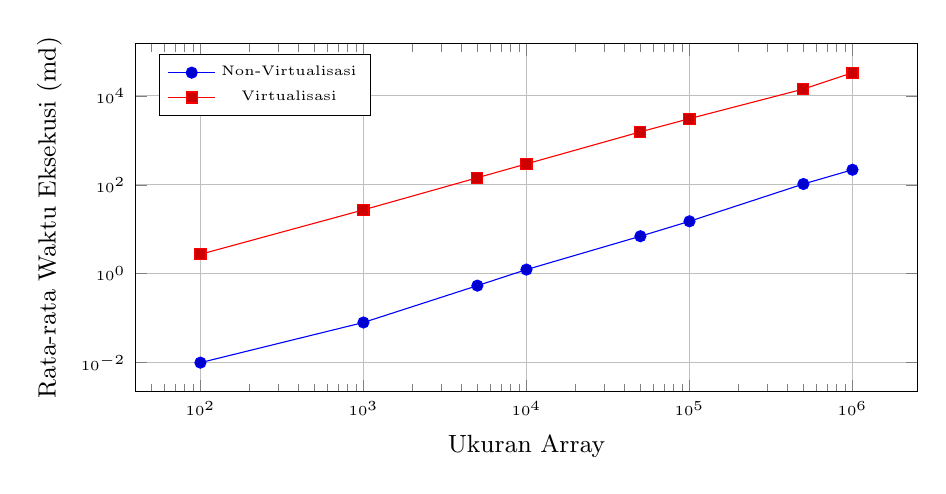
\begin{tikzpicture}
            \begin{axis}[
                    width=0.95\textwidth, height=6cm,
                    xlabel={Ukuran Array}, ylabel={Rata-rata Waktu Eksekusi (md)},
                    xmode=log, log basis x={10}, ymode=log, log basis y={10},
                    legend pos=north west, grid=major,
                    tick label style={font=\tiny}, label style={font=\small}, legend style={font=\tiny} ]
                \addplot coordinates { (100, 0.01) (1000, 0.08) (5000, 0.54) (10000, 1.24) (50000, 6.98) (100000, 15.12) (500000, 104.44) (1000000, 218.32) };
                \addlegendentry{Non-Virtualisasi};
                \addplot coordinates { (100, 2.74) (1000, 27.35) (5000, 144.44) (10000, 295.77) (50000, 1556.15) (100000, 3080.30) (500000, 14298.92) (1000000, 33292.91) };
                \addlegendentry{Virtualisasi};
            \end{axis}
        \end{tikzpicture}
        \caption{Perbandingan Waktu Eksekusi Quick Sort (Skala Log-Log).}
        \label{fig:quick_sort_performance_jurnal_ui_ana}
    \end{figure}

    \item \bo{Enkripsi AES:} Tabel \ref{tab:aes_performance_jurnal_ui_ana} menunjukkan bahwa total waktu untuk mengenkripsi 976MB data meningkat sekitar 396.7\% (1878.52 md menjadi 9330.73 md), dan waktu dekripsi meningkat sekitar 562.9\% (1304.75 md menjadi 8649.74 md). Akibatnya, \f{throughput} gabungan turun drastis dari 634.16 MB/s menjadi 108.78 MB/s (penurunan 82.8\%).
    % CATATAN: Anda perlu MENGISI DATA dari Tabel 5.6 dari skripsi Anda,
    % dan menyesuaikan label tabelnya menjadi unik untuk jurnal ini.
    \begin{table}[H]
        \centering
        \caption{Hasil Performa AES-256-CBC (Data 976MB)}
        \label{tab:aes_performance_jurnal_ui_ana}
        \fontsize{12}{12}\selectfont % Atur font size 10pt untuk tabel ini
        % SALIN KONTEN TABEL 5.6 DARI SKRIPSI ANDA KE SINI
        \begin{tabular}{@{}lrr@{}}
            \toprule
            \textbf{Metrik}              & \textbf{Non-Virtualisasi} & \textbf{Virtualisasi} \\
            \midrule
            Total Waktu Enkripsi (md)   & 1.878.52                 & 9.330.73             \\
            Total Waktu Dekripsi (md)   & 1.304.75                 & 8.649.74             \\
            % ... (Lanjutkan dengan data lainnya) ...
            Throughput Gabungan (MB/s)   & 634.16                   & 108.78               \\
            \bottomrule
        \end{tabular}
    \end{table}
\end{itemize}

\subsubsection{\f{Overhead} Ukuran Berkas}
Tabel \ref{tab:file_size_jurnal_ui_ana} menunjukkan peningkatan konsisten ukuran \f{executable} setelah virtualisasi. Untuk program konsol/benchmark yang lebih kecil, ukurannya meningkat lebih dari 15-18 kali lipat. Untuk aplikasi GUI yang lebih besar, peningkatan relatif lebih kecil namun tetap signifikan.
% CATATAN: Anda perlu MENGISI DATA dari Tabel 5.7 dari skripsi Anda,
% dan menyesuaikan label tabelnya menjadi unik untuk jurnal ini.
\begin{table}[H]
    \centering
    \caption{Perbandingan Ukuran Berkas Executable (KB)}
    \label{tab:file_size_jurnal_ui_ana}
    \fontsize{12}{12}\selectfont % Atur font size 10pt untuk tabel ini
    % SALIN KONTEN TABEL 5.7 DARI SKRIPSI ANDA KE SINI
    \begin{tabular}{@{}lrr@{}}
        \toprule
        \textbf{Program}  & \textbf{Non-Virtualisasi (KB)} & \textbf{Virtualisasi (KB)} \\
        \midrule
        quick\_sort       & 98                            & 1.537                     \\
        % ... (Lanjutkan dengan data lainnya) ...
        Lilith\_Client    & 84                            & 1.554                     \\
        \bottomrule
    \end{tabular}
\end{table}

\subsection{Diskusi}
Hasil eksperimen dengan jelas menunjukkan \textit{trade-off} inti dalam penggunaan virtualisasi kode VxLang.

\bo{Peningkatan Keamanan dan Penghindaran Deteksi:} VxLang memberikan penghalang substansial terhadap teknik rekayasa balik umum. Transformasi menjadi \f{bytecode} yang diinterpretasi menetralisir alat analisis statis standar seperti Ghidra \cite{Eilam2011, Ko2007} dan secara signifikan mempersulit analisis dinamis dengan alat seperti x64dbg, karena logika yang mendasarinya dieksekusi oleh VM buram \cite{Sikorski2012}. Hal ini sejalan dengan pemahaman mapan bahwa pengaburan berbasis VM secara fundamental mengubah struktur kode di luar kemampuan interpretasi \f{disassembler} standar \cite{Ore06, Salwan2018SymbolicDeobfuscation}. Lebih lanjut, analisis VirusTotal terhadap sepuluh sampel \f{malware}/PUA mengungkapkan dampak yang bernuansa: sementara VxLang dapat mengurangi deteksi berbasis \f{signature} untuk beberapa sampel, ia menyebabkan peningkatan deteksi untuk sampel lain, kemungkinan karena lapisan virtualisasi itu sendiri ditandai. Ini menyoroti interaksi kompleks antara pengaburan dan heuristik deteksi AV yang berkembang \cite{Ore06, Salwan2018SymbolicDeobfuscation, Rou13}.

\bo{Biaya Performa:} Manfaat keamanan dan penghindaran deteksi datang dengan harga performa yang mahal. \f{Overhead} interpretasi secara signifikan memperlambat kode tervirtualisasi, terutama untuk tugas-tugas komputasi intensif (\f{overhead} QuickSort ~15.000\% untuk 1 juta elemen; pengurangan \f{throughput} AES ~83\%), yang berpotensi membuat aplikasi yang tidak pandang bulu menjadi tidak praktis karena degradasi kecepatan yang parah.

\bo{Peningkatan Ukuran:} Peningkatan ukuran berkas yang cukup besar (misalnya, 15-18x untuk aplikasi kecil), terutama karena \textit{runtime} VM yang disematkan, merupakan faktor lain, khususnya relevan untuk aplikasi kecil atau kendala distribusi.

\bo{Implikasi Praktis:} VxLang tampak ampuh untuk melindungi kode yang sangat sensitif di mana keamanan dan potensi penghindaran deteksi adalah yang terpenting, dan dampak performa pada segmen spesifik tersebut dapat diterima (misalnya, anti-\f{tamper}, lisensi, IP inti). Kasus Lilith menunjukkan bahwa VxLang dapat melindungi logika kompleks tanpa merusaknya, \textbf{asalkan penempatan makro dilakukan dengan hati-hati dan iteratif untuk menghindari gangguan fungsionalitas, terutama pada bagian kode dengan alur kontrol kompleks atau operasi I/O}. Namun, biaya performa yang parah mengharuskan aplikasi strategis dan selektif, hanya menargetkan bagian kritis. Hasil VirusTotal juga menyiratkan bahwa meskipun profil deteksi diubah, penghindaran tidak dijamin. Pilihan antara autentikasi \f{hardcoded} dan berbasis \f{cloud} menunjukkan bahwa melindungi logika sisi klien yang menangani hasil validasi tetap krusial.
     % (results_discussion.tex)
% journal_ui_ana/english/src/50_kesimpulan.tex
\section{Conclusion}
\label{sec:conclusion_jurnal_ui_ana_en_condensed}

This study investigated the effectiveness of code virtualization using the VxLang framework to complicate software reverse engineering. Implementation involved marking source code, compiling intermediate executables, and processing them with the VxLang tool to generate virtualized binaries.

Experimental analysis demonstrated that VxLang's code virtualization significantly increases the difficulty of reverse engineering. Static analysis using Ghidra on virtualized code failed to identify meaningful instructions, functions, or data structures. Similarly, dynamic analysis with x64dbg was hampered by obfuscated control flow and the virtual machine's (VM) execution model, which obscured runtime behavior and debugging attempts. Efforts to bypass authentication logic, trivial in non-virtualized versions, were successfully thwarted in VxLang-protected binaries. However, effective implementation requires careful and iterative placement of virtualization macros, as improper placement, especially in code with I/O or complex control flows, can disrupt application functionality, as observed in the Lilith RAT case study.

Analysis of ten malware/PUA samples on VirusTotal showed varied impacts of VxLang on detection rates: approximately half of the samples exhibited a decrease in detections, often with a shift to generic/heuristic flags, while the remainder showed an increase in detections, indicating the virtualization layer itself can trigger alerts.

This enhanced security comes with substantial performance overhead, observed in QuickSort algorithm and AES encryption benchmarks, along with a significant increase in executable file size. The findings underscore a clear trade-off: strong protection against reverse engineering at the cost of performance degradation and increased file size. Therefore, practical application of VxLang should likely be selective, targeting only the most critical and sensitive code sections.

Future research could focus on exploring more advanced reverse engineering techniques against VM-based protections, investigating VxLang configuration options for security-performance balance, and comparative studies with other virtualization solutions. Deeper analysis of VxLang's interaction with various malware types and antivirus detection techniques would also yield valuable insights.
           % (conclusion.tex)
% \input{src/acknowledgment.tex} % Jika ada

% --- Daftar Pustaka ---
\clearpage
\begin{singlespace} % Biasanya referensi spasi tunggal
    \fontsize{10}{12}\selectfont % Font TNR 10 untuk referensi
    \printbibliography[heading=bibintoc, title={\fontsize{10}{12}\textbf{REFERENSI}}]
    % Atau jika ingin tanpa nomor section dan bold:
    % \printbibliography[heading=none, title=\centerline{\fontsize{10}{12}\selectfont\textbf{REFERENCES}}]
\end{singlespace}

\end{document}
